\documentclass[a4paper,11pt]{article}
\input{/home/tof/Documents/Cozy/latex-include/preambule_lua.tex}
\newcommand{\showprof}{show them}  % comment this line if you don't want to see todo environment
\fancyhead[L]{Missile Patriot - Nombres flottants}
\newdate{madate}{10}{09}{2020}
\fancyhead[R]{Première - NSI} %\today
\fancyfoot[L]{~\\Christophe Viroulaud}
\fancyfoot[C]{\textbf{Page \thepage}}
\fancyfoot[R]{\includegraphics[width=2cm,align=t]{/home/tof/Documents/Cozy/latex-include/cc.png}}
\usepackage{tikz}

\begin{document}
\begin{Form}
\paragraph{Objectif:}Comprendre la représentation des nombres réels en mémoire.
\section{Problématique}
Le 25 février 1991, à Dharan en Arabie Saoudite, un missile Patriot (figure \ref{patriot}) américain a raté l’interception d’un missile Scud irakien, ce dernier provoquant la mort de 28 personnes. La commission d'enquête a conclu à un défaut de l'horloge interne du missile. Cette dernière mesurait le temps en~1/10s.
\begin{figure}[!h]
\centering
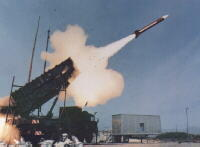
\includegraphics[width=5cm]{ressources/patriot.jpg}
\captionof{figure}{Missile Patriot}
\label{patriot}
\end{figure}
\begin{center}
\shadowbox{\parbox{13cm}{\centering Pourquoi la représentation en mémoire du temps a engendré cette erreur?}}
\end{center}
\section{Représentation générale des nombres réels}
\subsection{Écriture scientifique}
L'écriture scientifique des nombres réels répond à certaines règles:
\begin{itemize}
\item $1468=+1,468×10^3$
\item $-891=-8,91×10^2$
\item $0,00023=2,3×10^{-4}$
\end{itemize}
La forme générale s'écrit:
$$\pm 1×mantisse×10^{exposant}$$
\subsection{Représentation en mémoire}
La représentation des nombres réels en mémoire s'appuie sur l'écriture scientifique mais:
\begin{itemize}
\item elle utilise la \emph{base 2},
\item l'exposant est \emph{biaisé} (décalé) d'une valeur \emph{d} dépendante du format (32 ou 64 bits),
\item la mantisse est comprise entre [1;2[.
\end{itemize}
La forme générale s'écrit:
$$(-1)^s×m×2^{n-d}$$
\section{La norme \emph{IEE 754}}
\subsection{Les choix effectués}
C'est une norme mise au point par le \emph{Institute of Electrical and Electronics Engineers}. Des choix techniques ont été pris:
\begin{itemize}
\item Cette représentation n'utilise pas le \emph{complément à 2} pour stocker les exposants négatifs, mais un décalage d'une valeur \emph{d}.
\item La mantisse est un nombre de la forme 1,xxxxxx. Afin de gagner 1 bit en précision, on ne représente que les chiffres après la virgule.
\end{itemize}
\subsection{Les formats}
\begin{itemize}
\item \emph{Simple précision:} Le nombre est représenté sur 32 bits.
\begin{center}
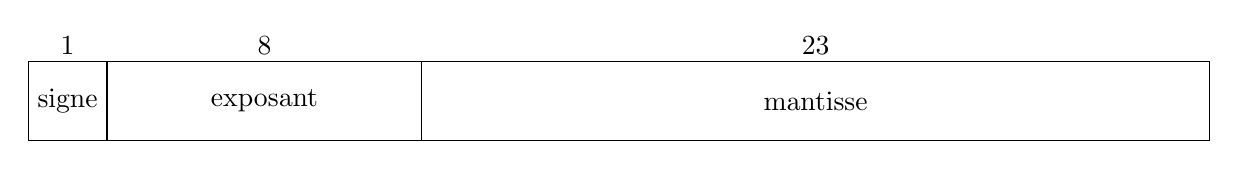
\begin{tikzpicture}
\draw (0,0) rectangle (1,1);
\draw (0.5,0.5) node {signe} ;
\draw (0.5,1.2) node {1} ;
\draw (1,0) rectangle (5,1);
\draw (3,0.5) node {exposant} ;
\draw (3,1.2) node {8} ;
\draw (5,0) rectangle (15,1);
\draw (10,0.5) node {mantisse} ;
\draw (10,1.2) node {23} ;
\end{tikzpicture}
\end{center}
L'exposant est représenté sur 8 bits donc des entiers entre 0 et 255. Il est décalé de \emph{d=127} donc il est possible de représenter des exposants \emph{signés} dans l'intervalle [-127;128].
\item \emph{Double précision:} Le nombre est représenté sur 64 bits.
\begin{center}
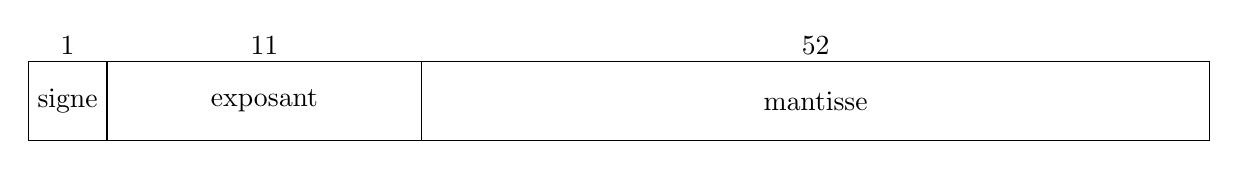
\begin{tikzpicture}
\draw (0,0) rectangle (1,1);
\draw (0.5,0.5) node {signe} ;
\draw (0.5,1.2) node {1} ;
\draw (1,0) rectangle (5,1);
\draw (3,0.5) node {exposant} ;
\draw (3,1.2) node {11} ;
\draw (5,0) rectangle (15,1);
\draw (10,0.5) node {mantisse} ;
\draw (10,1.2) node {52} ;
\end{tikzpicture}
\end{center}
\end{itemize}
\begin{activite}
\begin{enumerate}
\item En s'appuyant sur le format 32 bits, donner la valeur du décalage \emph{d} pour le format 64 bits.
\item En déduire les valeurs possibles pour l'exposant.
\end{enumerate}
\begin{commentprof}
$2^{11} = 2048$ donc entre 0 et 2047 nombres\\
$d = 2^{11-1}-1=1023$ donc exposants signés dans [-1023; 1024]
\end{commentprof}
\end{activite}
\subsection{Un exemple}
Considérons le mot de 32 bits:
$$\overbrace{1}^{signe}\overbrace{10000110}^{exposant}\overbrace{10101101100000000000000}^{mantisse}$$
\begin{itemize}
\item signe: $(-1)^1=-1$
\item mantisse: $1+2^{-1}+2^{-3}+2^{-5}+2^{-6}+2^{-8}+2^{-9} = 1,677734375$
\item exposant: $(2^7+2^2+2^1)-127=134-127=7$
\end{itemize}
Le nombre représenté est:
$$-1×1,677734375×2^7=-214,75$$
\subsection{Pour aller plus loin}
La norme \emph{IEEE 754} contient davantage de subtilités (représentation de 0, infini, dépassement de capacité, écart minimal...). Cette notion n'est pas au programme mais il peut être intéressant de lire la page Wikipédia correspondante:
\begin{center}
\url{https://fr.wikipedia.org/wiki/IEEE_754}
\end{center} 
\section{Limites de la représentation}
\subsection{Convertir un nombre réel}
\begin{activite}
\begin{enumerate}
\item En s'aidant de la page web \url{https://tinyurl.com/yyeymmln}, convertir 0,6875 en base~2.
\item Donner alors la représentation \emph{en simple précision} de ce nombre.
\end{enumerate}
\begin{commentprof}
$0,1011=1,011×2^{-1}$\\signe: 0\\mantisse: 011000....\\exposant: $-1+127=126_{10}=01111110_2$
\end{commentprof}
\end{activite}
\subsection{Erreur de calcul?}
Le code ci-après renvoie un résultat surprenant.
\begin{lstlisting}
>>> 0.1+0.2
\end{lstlisting}
Essayons d'expliquer ce résultat.
\begin{activite}
\begin{enumerate}
\item Convertir 0,2 en base 2.
\item Que peut-on en déduire sur la représentation de ce nombre en mémoire?
\end{enumerate}
\end{activite}
\section{Imprécision du missile Patriot}
L’horloge interne du missile Patriot mesure le temps en 1/10s soit 0,1s. Pour obtenir le temps en seconde, le système multipliait ce nombre par 10 en utilisant un registre de 24 bits en virgule fixe. 
\begin{activite}
\begin{enumerate}
\item Convertir 0,1 en base 2. Que constate-t-on?
\end{enumerate}
Le registre de 24 bits contenait $(0,00011001100110011001100)_2$ et induisait une erreur binaire de $(0,0000000000000000000000011001100...)_2$, soit approximativement 0,000000095s en notation décimale.
\begin{enumerate}[resume]
\item Le missile était allumé depuis 100 heures. Calculer le décalage \emph{noté \varepsilon} entre l'horloge interne et le temps réel.
\item Un missile Scud volait à la vitesse de $1676m.s^{-1}$. Calculer la distance parcourue par le missile pendant la durée \varepsilon.
\end{enumerate}
\end{activite}
\begin{commentprof}
0,000000095×100×3600×10=0,34s\\
1676×0,34 = 569m
\end{commentprof}
\end{Form}
\end{document}